\chapter{Lecture 24 - Convection in Rod Bundles}
\label{ch:ch24}
\section{Objectives}
The objectives of this lecture are:
\begin{enumerate}
\item Present relevant correlations to characterize convective heat transfer in arrays of cylindrical fuel pins.
\item Apply the correlation in a simple example problem
\end{enumerate}

\section{Convective Heat Transfer in Rod Bundles}

\newthought{As one might guess,} rod bundles must be handled differently than circular tubes for heat transfer. Similar to hydraulic analysis, convective heat transfer performance around a fuel pin in a fuel bundle depends on a number of factors such as:

\begin{marginfigure}
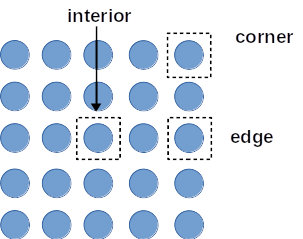
\includegraphics{assy_position.png}
\caption{Schematic of fuel pin positions within a fuel assembly.}
\end{marginfigure}

\begin{enumerate}
\item whether the fuel assembly is rectangular/square or triangular/hexagonal.  
\item the spacing between adjacent fuel pins---non-dimensionalized, as usual, as the pitch-to-diameter ratio.
\item the position of the pin within the fuel assembly---i.e. whether the pin is on an assembly edge, corner, or somewhere in the middle.
\end{enumerate} 


Also, as was the case for hydraulic analysis, one must substitute characteristic dimensions such as pipe diameter, with a more generic hydraulic diameter calculated from:
\begin{equation}
D_h = \frac{4 A_{\text{flow}}}{P_{\text{wetted}}}
\label{eq:hyd_diameter_24}
\end{equation}
where, as a reminder, flow area and wetted perimeter in coolant channels around fuel pins in rectangular and hexagonal arrays are illustrated in Figure \ref{fig:equi_ann_24}.
\index{hydraulic diameter}
\begin{marginfigure}
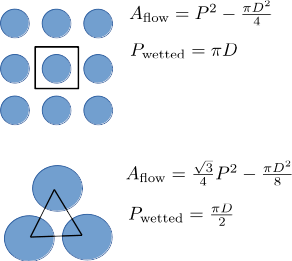
\includegraphics{equiv_annulus.png}
\caption{$A_{\text{flow}}$ and $P_{\text{wetted}}$ in fuel assemblies.}
\label{fig:equi_ann_24}
\end{marginfigure}


\newthought{The customary method} with correlations for convective heat transfer in a rod bundle will be to express the Nusselt number in terms of the Nusselt number for fully developed turbulent flow in a circular channel as shown in Equation \ref{eq:conv1_24}

\begin{equation}
\text{Nu}_{\infty} = \psi \left(\text{Nu}_{\infty} \right)_{\text{c.t.}}
\label{eq:conv1_24}
\end{equation}
where, of course, $(\text{Nu}_{\infty})_{\text{c.t.}}$ is the Nusselt Number for a circular tube which, unless otherwise stated, should be calculated using the Dittus-Boelter correlation.  Consequently, the correlations to be presented are meant to specify a value for $\psi$.

\section{Infinte Arrays}
For an ``infinite array'' of rods, what we really mean is that all rods are treated as interior rods; there are no corners or boundaries in an infinite array and thus no corner or edge fuel cooling channels.

\subsection{Presser Correlation}\index{Presser correlation}
Presser and his colleagues provided correlations for both hexagonal and square arrays.

Hexagonal arrays:
\begin{equation}
\psi = 0.9090 + 0.0783 \frac{P}{D} - 0.1283 e^{-2.4(\sfrac{P}{D}-1)}
\label{eq:presser-hex}
\end{equation}
for $1.05 \le \sfrac{P}{D} \le 2.2$.

For square arrays:
\begin{equation}
\psi = 0.9217 + 0.1478 \frac{P}{D} - 0.1130 e^{-7.0(\sfrac{P}{D} - 1)}
\label{eq:presser-square}
\end{equation} 
for $1.05 \le \sfrac{P}{D} \le 1.9$

\subsection{Weisman Correlation} \index{Weisman correlation}
For the special case of water-cooled applications, Weisman provides a correlation.\cite{weisman1959heat}

For hexagonal arrays:

\begin{equation}
\psi = 1.130 \frac{P}{D} - 0.2609
\end{equation}
for $1.1 < \sfrac{P}{D} < 1.5$.

For square arrays:
\begin{equation}
\psi = 1.826 \frac{P}{D} - 1.0430
\end{equation}
for $1.1 \le \sfrac{P}{D} \le 1.3$.

\section{Finite Arrays}
Correlations for finite arrays generally incorporate some mechanism to account for the fuel rod location within the assembly.  As previously discussed, a reasonably simple model will consider only three cases: a rod on the edge, corner, or interior or the assembly.  

The one correlation of this type that we will consider is from Markoczy.\cite{markoczy1972convective}  The basic correlation is given by Equation \ref{eq:markoczy}

\begin{equation}
\psi = 1 + 0.9120 \text{Re}^{-0.1} \text{Pr}^{0.4} \left(1 - 2.0043 e^{-B} \right)
\label{eq:markoczy}
\end{equation}
where the parameter $B$ is given by:
\begin{equation}
B = \frac{D_e}{D}
\end{equation}
where, in turn, $D_e$ is given by:
\begin{equation}
D_e = 4 \frac{\sum_j A_j}{\sum_j P_{\text{wetted},j}}
\end{equation}
where $A_j$ and $P_{\text{wetted},j}$ are the flow area and wetted perimeter of all flow channels adjacent to the rod.  This is where the effect of a finite array can be seen.

In the case of a typical interior rod---where all of the adjacent channels are the same and which for this class is the only case we will consider---the equation for $B$ reduces to:

\begin{equation}
B = \frac{2 \sqrt{3}}{\pi}\left(\frac{P}{D} \right)^2 - 1
\end{equation}
for triangular arrays, and:

\begin{equation}
B = \frac{4}{\pi}\left(\frac{P}{D} \right)^2 - 1
\end{equation}
for square arrays.

\section{Example}
Consider a typical fuel assembly for an AP1000 core.  The fuel pins are arranged in a 17x17 square array.  Each fuel pin has an outside diameter of 0.374 inches and a rod pitch of 0.496 inches. Coolant flows through the average channel with a velocity of 15.9 ft/sec. Coolant properties are as given in Table \ref{tab:example_ch24}

\begin{margintable}
\begin{tabular}{l c}
\toprule
Property & Value \\
\hline
Average $\rho$ [lb$_m$/ft$^3$] & 45.2 \\
Average $\mu$ [lb$_m$/ft-hr] & 0.23 \\
Average $c_p$ [BTU/lb$_m$-R] & 1.31 \\
Average $k$ [BTU/hr-ft-R] & 0.32\\
\bottomrule
\end{tabular}
\caption{Fluid properties for Lecture 24 example.}
\label{tab:example_ch24}
\end{margintable}

\vspace{0.5 cm}
\textbf{Find:}
\begin{enumerate}
\item Nusselt number using Dittus-Boelter correlation.
\item Nusselt number and convective heat transfer coefficient using
\begin{enumerate}
\item Presser correlation
\item Markoczy correlation for an interior channel
\end{enumerate}
\item The temperature at the clad surface at a location in the channel where the bulk coolant temperature is 580$^{\circ}$F and the heat flux is 346,104 BTU/hr-ft$^{2}$.  Use the convective heat transfer coefficient from the Markoczy correlation.
\end{enumerate}


\begin{fullwidth}
\subsection{Solution}
To use the correlations, we need to find the hydraulic diameter of the flow channel surrounding a typical interior fuel pin from the square array.
\begin{equation*}
A_f = P^2 - \frac{\pi}{4}D^2 = 0.496^2 - \frac{\pi}{4}(0.374)^2 = 0.1362 \text{in}^2 = 9.455 \times 10^{-4} \text{ ft}^2
\end{equation*}
\begin{equation*}
P_w = \pi D = \pi \left(\frac{0.374}{12} \right) = 0.09791 \text{ ft}
\end{equation*}

\begin{equation*}
D_h = \frac{4 A_f}{P_w} = \frac{4 (9.455 \times 10^{-4}}{0.09791} = 0.03863 \text{ ft}
\end{equation*}

With this we can calculate Reynolds number and, with given material properties Prandtl number
\begin{equation*}
\text{Re} = \frac{\rho v D_h}{\mu} = \frac{(45.2\  \text{lb}_m/\text{ft}^3)(15.9 \text{ ft/s})(0.03863 \text{ ft}}{0.23 \ \text{lb}_m\text{/ft-hr} \text{(1 hr/3600 sec)}} = 434,520
\end{equation*}

\begin{equation*}
\text{Pr} = \frac{\mu c_p}{k}= \frac{(0.23 \ \text{lb}_m\text{/ft-hr})(1.31 \text{ BTU/lb}_m\text{-R})}{0.32 \text{BTU/hr-ft-R}} = 0.\textbf{94}16
\end{equation*}

Now we can use the computed parameters in the specified correlations.

1. Dittus Boelter: $0.023 \text{Re}^{0.8}\text{Pr}^{0.4} = 0.023(434,545)^{0.8}(0.9416)^{0.4} = 727.3$

2.a Presser: $\phi\left( \right)_{\text{c.t}}$ where
$$ \phi = 0.9217 + 0.1478 \frac{P}{D} - 0.1130 e^{-7 \left(\sfrac{P}{D}-1 \right)}$$
where $\sfrac{P}{D} = \sfrac{0.496}{0.374} = 1.326$.  This gives a Nusselt number of 804.5

2.b Markoczy: the equations will not be repeated here, the resulting Nusselt number is 801.5

3. To answer this question we need to convert the Nusselt number that we got with the Markoczy correlation into a convective heat transfer coefficient.  From the definition of Nusselt number, we get:
$$h = \frac{\text{Nu} k}{D_h} = \frac{(801.5) (0.32 \text{ BTU/hr-ft-R})}{0.03863 \text{ ft}} = 6639 \text{ BTU/hr-ft}^{2}\text{-R}$$

$$\Delta T_{\text{cool}} = \frac{q^{\prime \prime}}{h} = \frac{364,104 \text{ BTU/hr-ft}^2}{6639 \text{ BTU/hr-ft}^{2}\text{-R}} =  52.1^{\circ}\text{R}$$

So the clad surface temperature is 580$^{\circ}$F + 52.1 $\approx$ 632$^{\circ}$F.
 

\end{fullwidth}
